\documentclass[11pt]{article}
\usepackage[T1]{fontenc}
\usepackage{latexsym,amssymb,amsmath,amsfonts,amsthm}
\usepackage{color}
\usepackage{tikz}
\usetikzlibrary{calc}
\usetikzlibrary{intersections,through}

\begin{document}

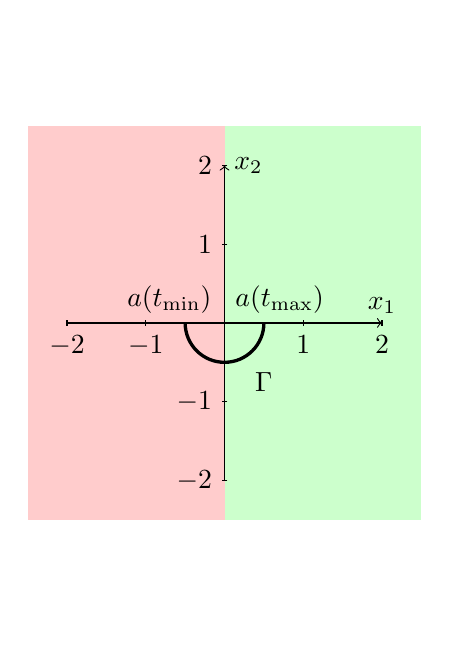
\begin{tikzpicture}
		\draw[line width=2.5cm,color=green!20] (1.25,-2.5) -- (1.25,2.5);
		\draw[line width=2.5cm,color=red!20] (-1.25,-2.5) -- (-1.25,2.5);
		\draw[->] (-2,0) -- (2,0) node[above] {$x_1$} coordinate(x axis);
		\draw[->] (0,-2) -- (0,2) node[right] {$x_2$} coordinate(y axis);
		\foreach \x/\xtext in {-2,-1, 1, 2}
		\draw[xshift=\x cm] (0pt,1pt) -- (0pt,-1pt) node[below] {$\xtext$};
		\foreach \y/\ytext in {-2,-1, 1, 2}
		\draw[yshift=\y cm] (1pt,0pt) -- (-1pt,0pt) node[left] {$\ytext$};

		\draw [very thick] (-0.5,0) arc [ start angle =180, end angle =360 ,radius =0.5];

		\draw (-0.7, 0) node [above] {$a(t_{\min})$};

		\draw (0.7, 0) node [above] {$a(t_{\max})$};

		\draw (0.5, -0.5) node [below] {$\Gamma$};
		


		\end{tikzpicture}

\end{document}